\begin{minipage}{0.46\textwidth} % Adjust the width of the image area
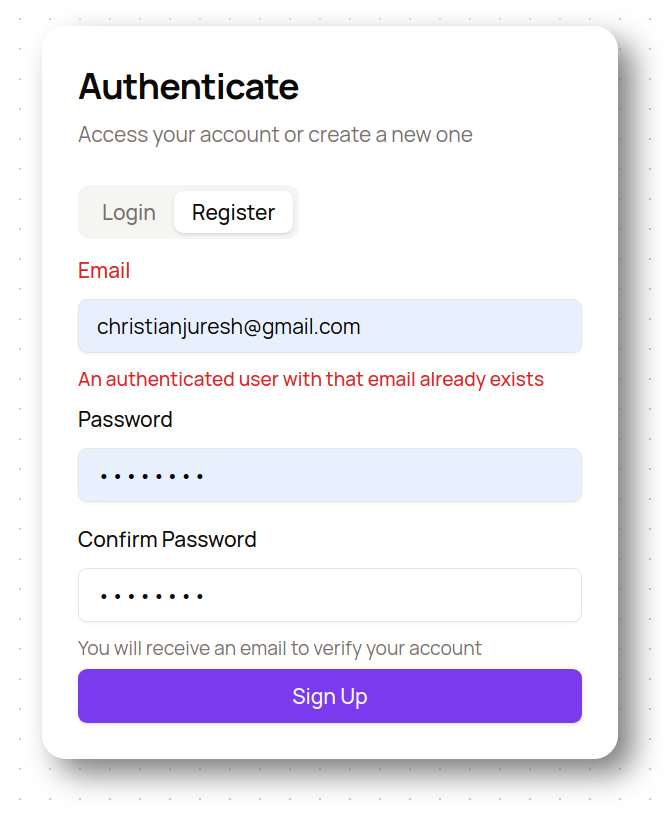
\includegraphics[width=\textwidth]{images/register.png} % Adjust the width as necessary, using \textwidth scales the image to fit the minipage
\end{minipage}
\hfill
\begin{minipage}{0.5\textwidth} % Adjust the width of the text area
\subsubsection{Registration}
    Users are met by an authentication page where they can choose to login or register. The registration form is validated in sveltekit using zod, and also communicates with the django backend to tell users if the email is already registered in the database. Upon registration, the user is sent an email by postmark to verify their account. When the link is pressed, the user is logged in and redirected to the profile page.
\end{minipage}

\vspace{0em}

\begin{minipage}[t]{0.47\textwidth} % Adjust the width of the text area
    \vspace{0.5em}
The schema in figure X is used to validate the registration form. It checks if the email is a valid email, and if the password and confirm\_password fields match. If the form is invalid, the user is shown an error message. 
\end{minipage}
\hfill
\begin{minipage}[t]{0.47\textwidth} % Adjust the width of the image area
\begin{minted}[
    frame=lines,
    framesep=2mm,
    fontsize=\scriptsize,
    breaklines,
    tabsize=2
    ]{typescript}
export const registerFormSchema = z
	.object({
		email: z.string().email(),
		password: z.string().min(8).max(50),
		confirm_password: z.string().min(8).max(50)
	})
	.refine((data) => data.password === data.confirm_password, {
		message: 'Passwords do not match',
		path: ['confirm_password']
	});

export type RegisterFormSchema = typeof registerFormSchema;
\end{minted}
\end{minipage}

\vspace{2em}

\begin{minipage}[t]{0.47\textwidth} % Adjust the width of the image area
\begin{minted}[
    frame=lines,
    framesep=2mm,
    fontsize=\scriptsize,
    breaklines,
    tabsize=2
    ]{typescript}
export const load: PageServerLoad = async (event) => {
	const token = event.cookies.get('token');
	if (token) {
		await axios
			.post('http://localhost:8000/api/token/verify', {
				token: token
			})
			.then(() => {
				redirect(302, '/protected/profile');
			});
	}

	return {
		loginForm: await superValidate(zod(loginFormSchema)),
		registerForm: await superValidate(zod(registerFormSchema))
	};
};
\end{minted}
\end{minipage}
\hfill
\begin{minipage}[t]{0.47\textwidth} % Adjust the width of the text area
    \vspace{0.5em}
The code in figure X occurs when the page loads. It checks if the user is already logged in with django-ninja-JWT, and if so, redirects them to the profile page. Otherwise, the login and registration schema are returned to be used in the frontend.
\end{minipage}


\begin{minipage}[t]{0.47\textwidth} % Adjust the width of the image area
\begin{minted}[
    frame=lines,
    framesep=2mm,
    fontsize=\scriptsize,
    breaklines,
    tabsize=2
    ]{typescript}
const sendVerificationEmail = async (email, token) => {
	const verificationUrl = `http://localhost:5173/auth/verify?token=${token}`;
	const client = new postmark.ServerClient('INSERT-SECRET-TOKEN-HERE');
	
	try {
		await client.sendEmail({
			From: 'verify@chrisj.uk',
			To: email,
			Subject: 'Verify your email',
			HtmlBody: `<strong>Please verify your email</strong> by clicking <a href="${verificationUrl}">here</a>.`,
			TextBody: `Please verify your email by visiting this link: ${verificationUrl}`,
			MessageStream: 'outbound'
		});
	} catch (error) {
		console.error('Failed to send verification email:', error);
		throw error;
	}
};
\end{minted}
\end{minipage}
\hfill
\begin{minipage}[t]{0.47\textwidth} % Adjust the width of the text area
    \vspace{0.5em}
    Here is the api for sending emails. The token from figure X is used in line 3 to create a verification url. The postmark server client is then used to send the email to the user.
\end{minipage}

\vspace{2em}

\begin{minipage}[t]{0.47\textwidth} % Adjust the width of the text area
    \vspace{0.5em}
    Users are initially registered as unauthenticated users, and are sent an email to verify their account. The code in figure X is used to handle the CRUD and storange of unauthenticated and authenticated users in the django backend.
\end{minipage}
\hfill
\begin{minipage}[t]{0.47\textwidth} % Adjust the width of the image area
\begin{minted}[
    frame=lines,
    framesep=2mm,
    fontsize=\scriptsize,
    breaklines,
    tabsize=2
    ]{python}
router = Router()
@router.post("/register-unauthenticated", url_name="register-unauthenticated")
def register_unauthenticated(request, user_in: UnauthenticatedUserIn):
    if user_exists(user_in.email):
        return HttpResponse("An authenticated user with that email already exists", status=400)
    else:
        create_unauthenticated_user(user_in.email, user_in.password, user_in.token)

@router.post("/register-validate", url_name="register-validate")
def register(request, user_in: TokenIn):
    unauth_user = get_object_or_404(UnauthenticatedUser, token=user_in.token)
    if user_exists(unauth_user.email):
        return HttpResponse("An authenticated user with that email already exists", status=400)
        
    with transaction.atomic():
        user = create_user(unauth_user.email, unauth_user.password)
        
        unauth_user.delete()

        tokens = get_token_for_user(user)

        return {
            'message': 'User registered successfully',
            'refresh': str(tokens),
            'access': str(tokens.access_token),
        }
\end{minted}
\end{minipage}